\subsection{Конфигурация на микроконтролера}

\subsubsection{Стартиране }

Написан е прост стартиращ скрипт на ARM assembly за целите на проекта, който инициализира SP на процесора и инициализира PC=Resethandler.
Скриптът дефинира символите от таблицата за прекъсванията, като .weak референции, към DefaultHandler, който изпълнява безкраен празен цикъл.
Този скрипт има за цел да инициализира .bss секцията на контролера,
както и всички статични променливи, като използва позициите, генерирани от линкерния скрипт, както и да извика функцията за системна инициализация, след което се извиква main финкцията.

\subsubsection{Системна инициализация}

В тази фаза се налага да бъде инициализиран системният часовник.
В нашия случай ще инициализираме системния часовник от високочестотният външен осцилатор (HSE). 
Тъй като при стартиране се използва високочестотният вътрешен осцилатор (HSI), който е
неточен и може да доведе до синхроннизационни проблеми при асинхронни комуникации 
с висок baud-rate като UART.
Поради тази причина се налага инициализирането на системния часовник с времева основа
високочестотният външен осцилатор (HSE), тъй-като е много по прецизен.
Високочестотният външен осцилатор (HSE) на платката е с честота 8MHz, затова използваме
хардуерният PLL модул за увеличаване на честотата със следните настройки:
\begin{verbatim}
    (PLL_M=8, PLL_N=336, PLL_P=2, PLL_Q=7)
\end{verbatim}
, като така получаваме  168MHz честота на системния часовник.
След това инициализираме делителите на честота за отделните шини:
\begin{verbatim}
    (AHB_Prescaler=1, APB1_Prescaler=4, APB2_Prescaler=2).
\end{verbatim}
След настройката на часовниците получаваме следните честоти за отделните шини (\autoref{fig:frequencies})

\begin{figure}[htpb!]
    \centering
    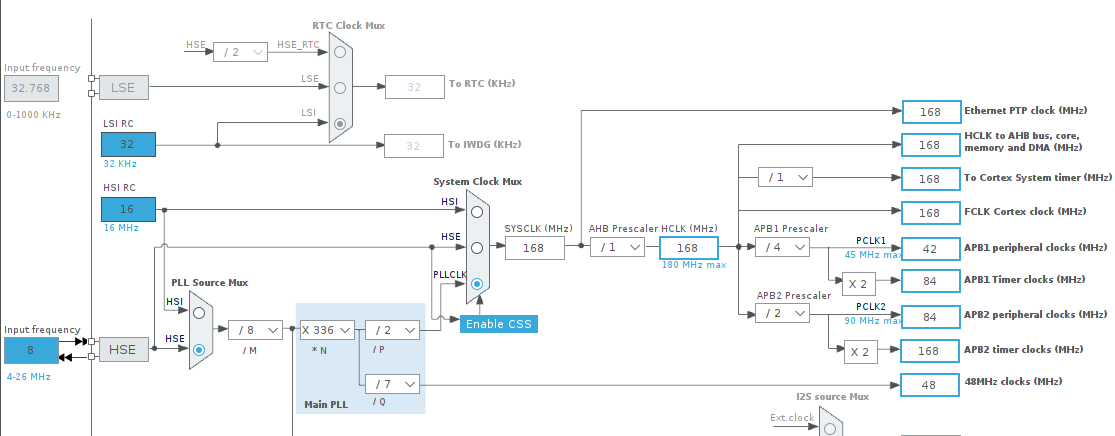
\includegraphics[width=0.9\textwidth]{frequencies}
    \caption{Честоти на системните шини и часовници след конфигурация}
    \label{fig:frequencies}
\end{figure}

Дуга основна част на системанта инициализация е инициализирането на хардуерния модул за числа с плаваща запетая (FPU).
Тъй като от конфигурацията (\autoref{lst:make_config}) настройваме комилатора за работа с модула за числа с плаваща запетая, е важно
преди която и да е операция с числа с плаваща запетая този модул да бъде инициализиран.
Необходимо е инициализацията на FPU да се случи преди преминването в ограничен режим.
Инициализацията се случва, чрез блокът от код (\autoref{lst:enable_fpu}).
\begin{lstlisting}[language=c, caption={Инициализация на модула за числа с плаваща запетая}, label={lst:enable_fpu}]
    /* Enable The FPU*/
    uint32_t* CPACR = (uint32_t*)0xE000ED88;
    *CPACR |=  0b00000000111100000000000000000000;
\end{lstlisting}

\subsubsection{Инициализация на периферията}

\change{WRITE}




